\chapter{Experiments}

% Short introduction such as: this chapter describes how the tests should be
% conducted, explain thorougly the scheduler script, gathered data etc.
\section{Proposed workflow and methodology}

In order to obtain the details of how system-level physical measurement
estimates energy consumption by a component (such as a CPU or a GPU)
during an application execution, several steps must be taken:

\begin{enumerate}
    \item Exclusive reservation of the entire computational node.
    \item Observation of the disk consumption and network usage before and
    during tests.
    \item Monitoring of the CPUs and GPUs utilization before and during tests.
    \item Running the benchmark kernels on an abstract processor only.
    Abstract processor comprises of the multicore CPU processor consisting
    of a certain number of physical cores and DRAM\@.
    \item Gathering of the power measurements.
    \item Verification of the accuracy and reliability of the software
    measurements tools, based on ground truth results.
\end{enumerate}

One of the notable mentions that could be done in order to reduce the amount
of uncertain power draw measurements done by the background components is
setting the fans to full speed. This solution have a potential of reducing
power draw fluctuations, especially during higher workloads, i\. e\. when
running benchmarks kernels utilizing maximum amount of GPUs or running Hybrid
configuration, where power draw of the entire nodes are very high. This could
not be implemented, however, as the administrator of the department's servers
stated, that interference in servers fans could be crucial for the nodes
stability.

\textbf{For Intel RAPL / NVIDIA Management Library:}
\begin{enumerate}
    \item Obtain base power of idle CPUs / GPUs.
    \item Obtain execution time of benchmark application.
    \item Obtain total energy consumption of the CPUs / GPUs during tests.
    \item Calculate dynamic energy consumption by subtracting base energy from
    total energy used during run.
\end{enumerate}

\textbf{For Yokotool:}
\begin{enumerate}
    \item Obtain base power of idle CPUs.
    \item Obtain execution time of benchmark application.
    \item Obtain total energy consumption of the CPUs during tests.
    \item Calculate dynamic energy consumption by subtracting base power from
    total energy used during run
\end{enumerate}

\newpage

In addition to the main experiments workflow, another methodology must be
adapted $-$ the data collection methodology. In order for the results to be
properly comparable, several point have to be met:
\begin{enumerate}
    \item Tests environment must be identical in every case, to eliminate
    discrepancy of the results.
    \item The results of the power draw reading must be properly compared for
    the device only measurements (Intel RAPL / NVML) and the measurements of
    the entire node (Yokotool).
    \item Experiments should be conducted on different nodes that utilizes
    different hardware, in order to state repeatability of tests. [TO BE REDACTED]
    \item Experiments should be conducted, using different benchmark kernels
    or application, to remove the possibility of bias of the results, due to
    poor diversification of test cases. [TO BE REDACTED]
    \item Test runs must be repeated many times.
\end{enumerate}

\section{Working environment $-$ servers details}

[PLACEHOLDER] NOTE: Probably this section will be cut, because it has been
covered in previous chapter
% Describe more thoroughly the nodes: CPUs, GPUs, RAM, PSUs, PM connection etc

\section{Main tests}

\subsection{Overview on the scheduler script}

In order to automate the experiments, an entire scheduler script had to be
created. Its has two main tasks: first is to store the information about the
configurations and run the benchmarks according to the presets. The second
is to run the measurements softwares and save all the results in the ordered
manner.

Both of these goals are reached by using dictionaries with key-value pairs.
That created a~tree-like dependencies between the corresponding layers of
configurations. Finally, that solution works for both choosing the right
config and providing the path to save measurements.


2. Section that run CPUs benchmarks, GPUs benchmarks, perf, nvml, yoko
3. Functions that check if the benchmarks are still running
4. Function that cleans-up every process after tests

\newpage

\subsection{Main automation function $-$ scheduler()}

% NOTE TO SELF: Make sure this chart belongs to this section

The entire scheduler script consists of classes and functions that are
explicitly designated for their purposes in the code. Overview of them is
as follows:

\begin{itemize}
    \item \textbf{class `Config'} $-$ Contains all the informations about the servers,
    devices, implementations, benchmarks and configurations, handles the
    relations between them and provides correct pathes to the corresponding
    measurements directories.
    \item \textbf{class `Benchmark'} $-$ Defines functions responsible for
    executing CPUs and GPUs benchmarks, as well as the measurements
    softwares: Linux Perf, NVIDIA Management Library and Yokotool
    \item \textbf{class `Execution'} $-$ This class contains functions tasked with
    calling the benchmark kernels and checking their status, if they are still
    running, for the purpose of ending the measurements. Since the
    measurements softwares are highly dependent on benchmarks being run, they
    are executed directly from the \emph{main\@()} function and
    the \emph{Execution} class only has the functions tasked with the proper
    termination of them.
    \item \textbf{function `scheduler\@()'} $-$ This major function triggers
    secondary functions from \emph{Execution} class and watched their status.
    \item \textbf{function `main\@()'} $-$ Runs every configuration
    sequentially, based on the lists of presets. Additionally, repeats every
    ten times in order to achieve repeatability of the experiments.
\end{itemize}

In order to visualize the entire workflow of the scheduler, as well as the 
workings of the individual processes, two charts has been created:
\begin{itemize}
    \item \textbf{General Flowchart} $-$ This chart
    (\textbf{Fig. \ref{fig:general_flowchart}}) describes the relations
    between the currently used configurations and the instructions executed
    based on those conditions.
    \item \textbf{Processes Flowchart} $-$ This chart
    (\textbf{Fig. \ref{fig:processes_flowchart}}) shows the working priciples of the
    \emph{runner\@()} subfunction, which shows the benchmarks and measurements
    softwares are started on a~high level of abstraction.
\end{itemize}

\newpage

\begin{figure}[hbtp!]
    \centering
    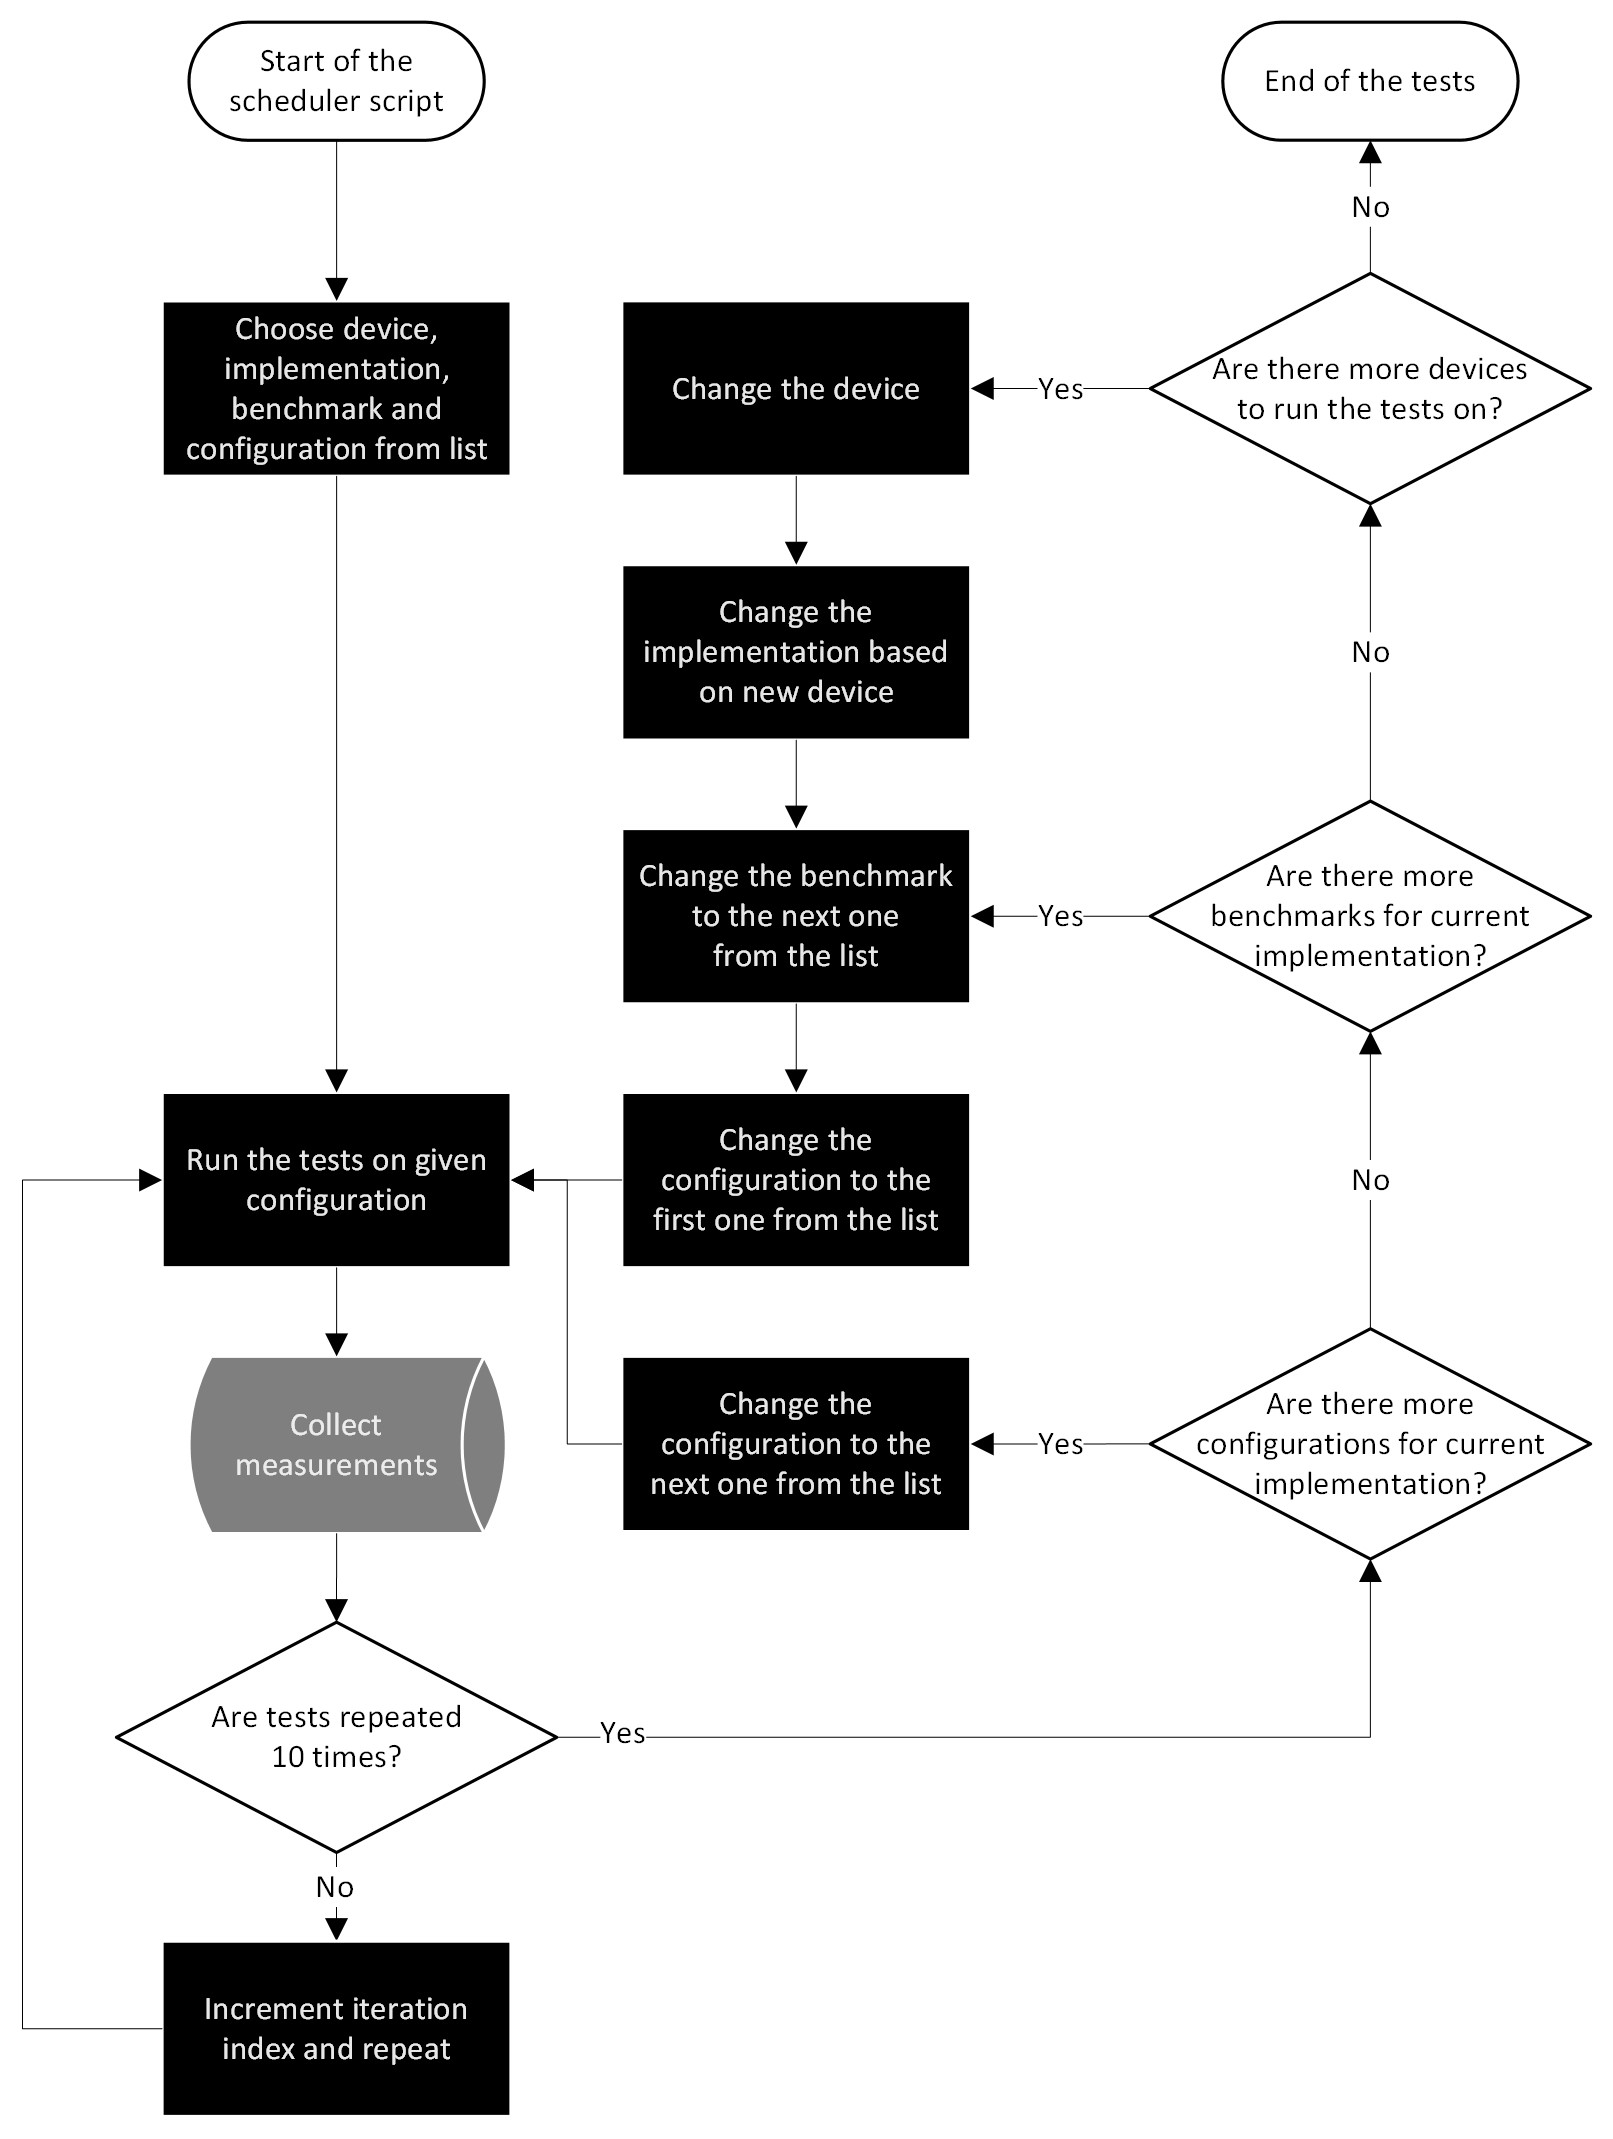
\includegraphics{general_flowchart}
    \caption{General Flowchart}~\label{fig:general_flowchart}
\end{figure}

\begin{figure}[hbtp!]
    \centering
    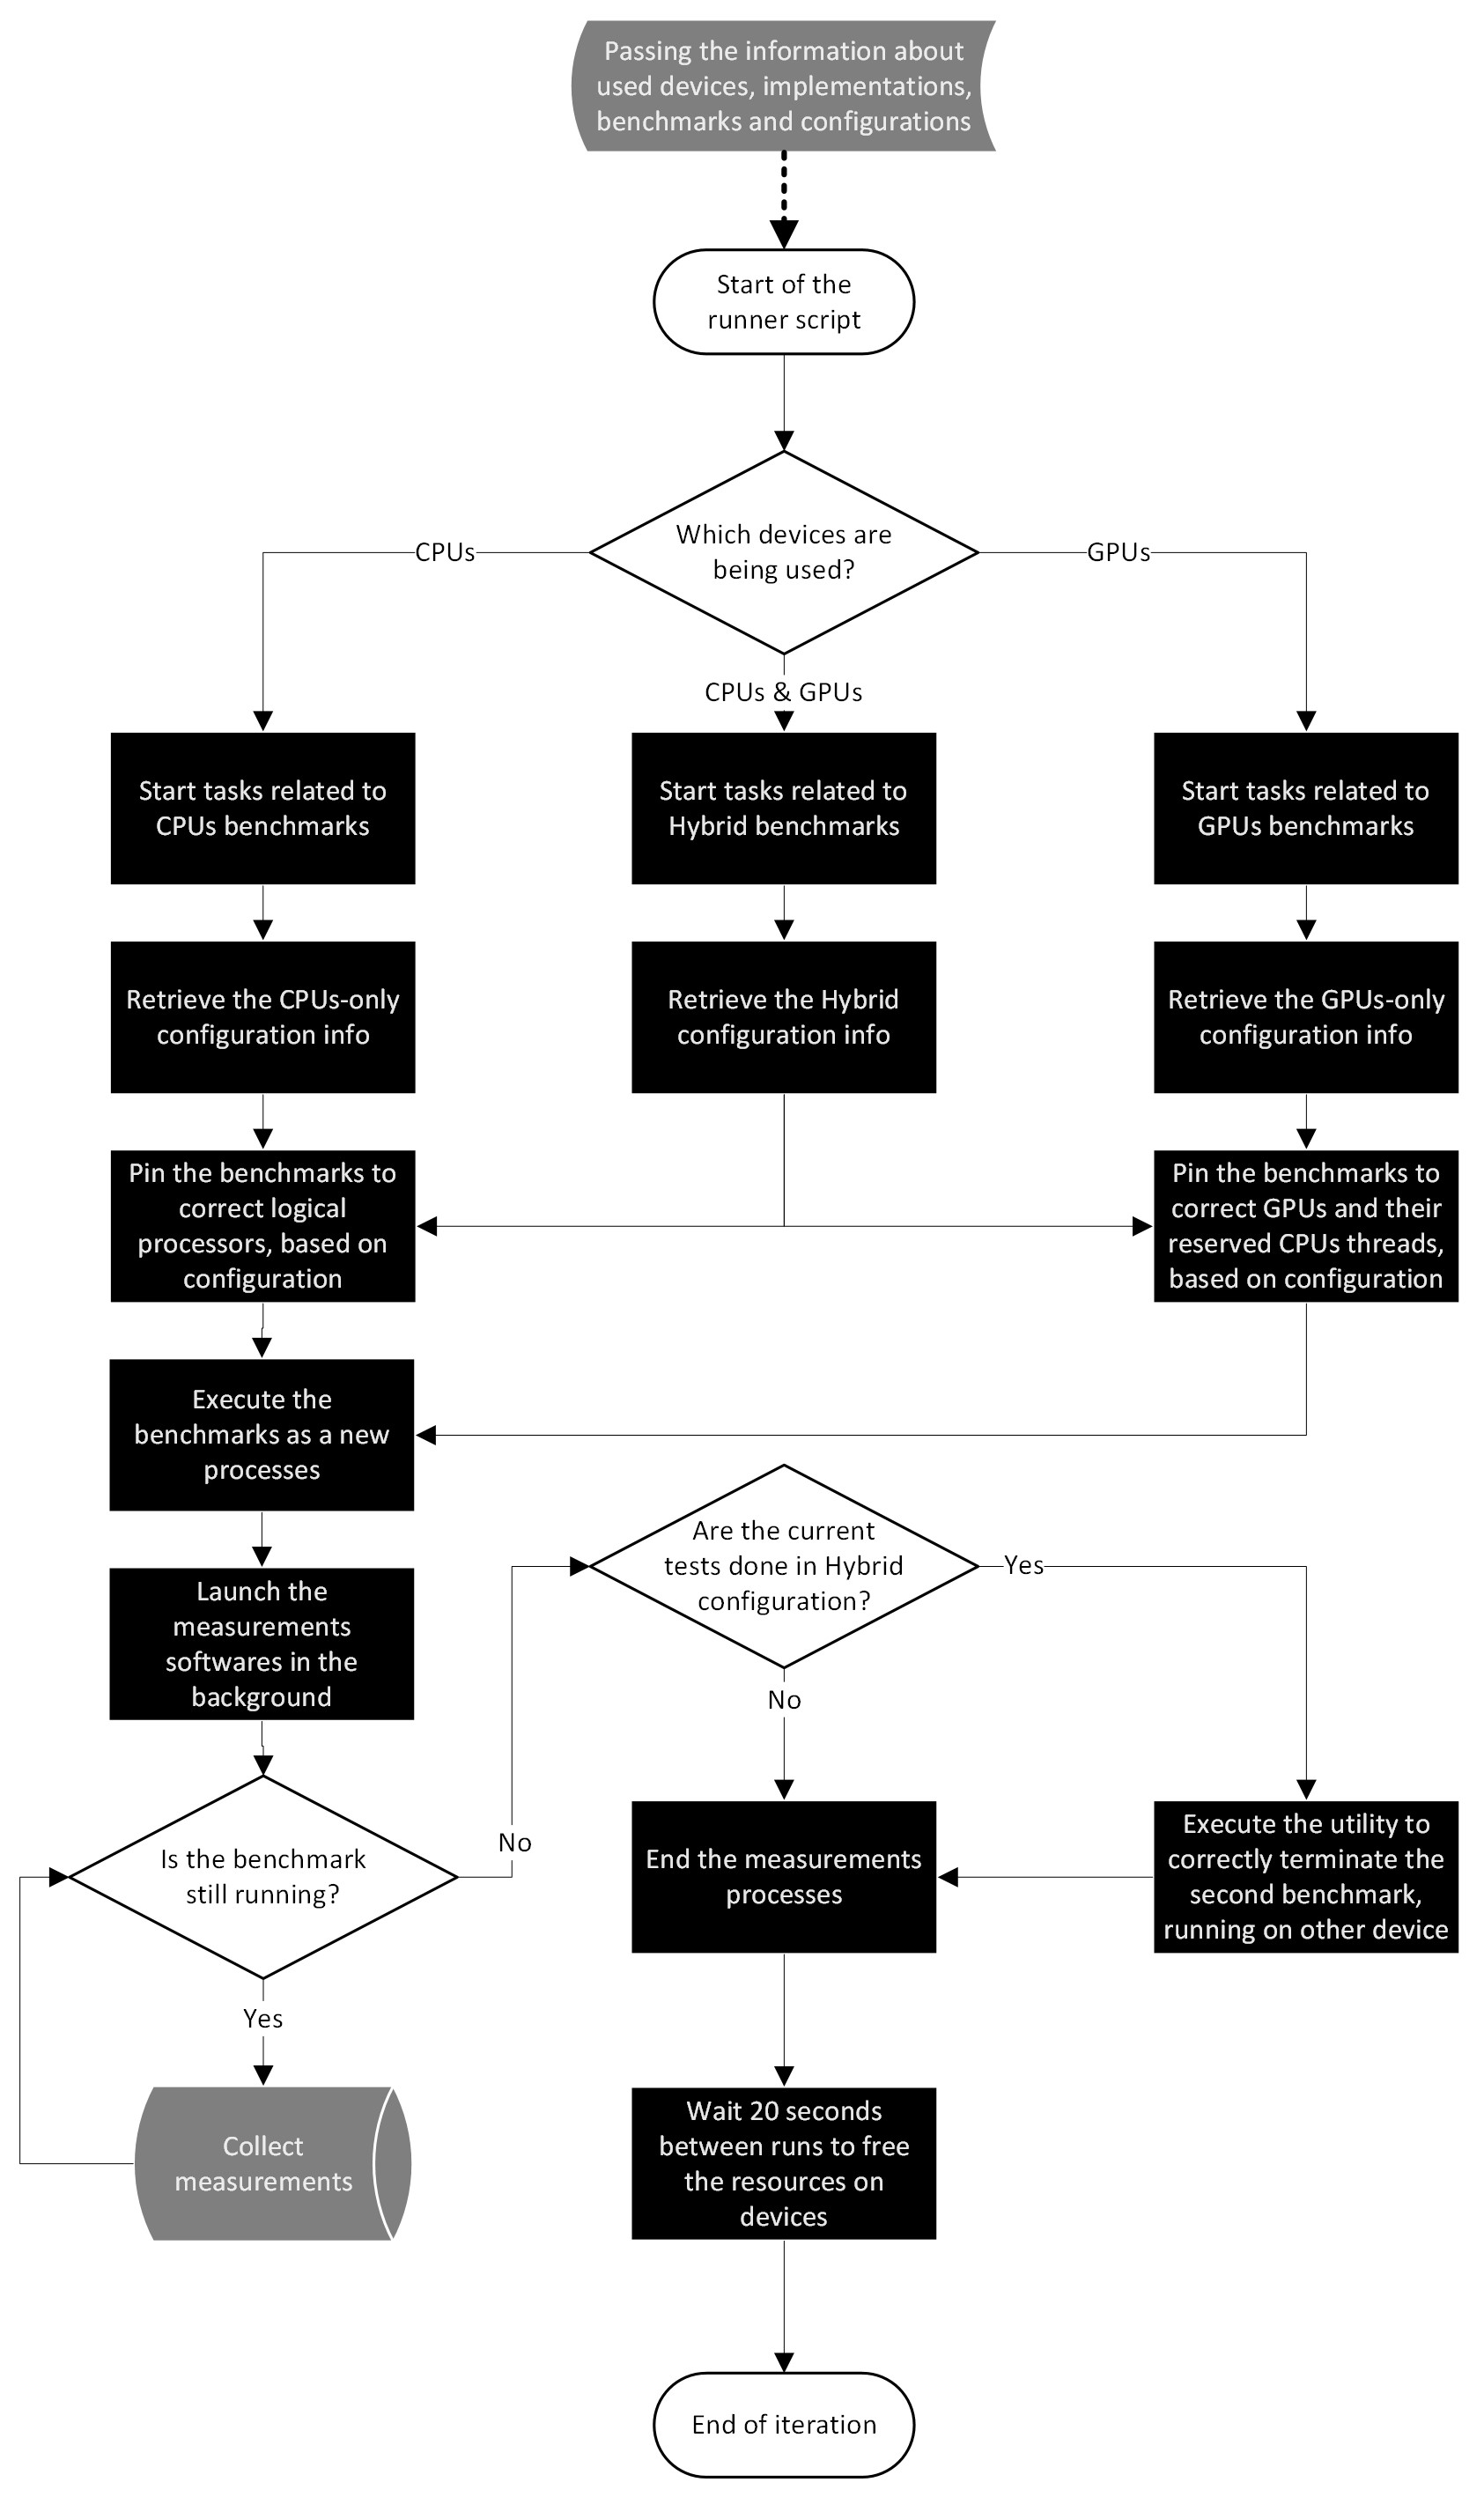
\includegraphics{processes_flowchart.jpeg}
    \caption{Processes Flowchart}~\label{fig:processes_flowchart}
\end{figure}

\newpage

\subsection{Threads pinning and kernels execution $-$ cpu\_benchmark()}

This function is responsible of executing CPUs benchmarks, based on the
given configuration. It creates a separate processes by utilizing the
Python \emph{subprocess} module. 

\begin{lstlisting}[language=Python]
    cpu_benchmark = subprocess.Popen(
        [
            "taskset --cpu-list <T> <P> <B> > /dev/null 2>&1"
        ],
        shell=True
    )
    return cpu_benchmark.pid
\end{lstlisting}

Here is an explanation of every part of the command:

\begin{itemize}
    \item \textbf{cpu\_benchmark} $-$ A variable of type
    \emph{<class `subprocess.Popen'>} is created mainly in order to
    retrieve PID later on.
    \item \textbf{subprocess.Popen} $-$ The underlying process creation and
    management is handled by the Popen class. Its function is to execute
    a child program in a new process.
    \item \textbf{taskset} $-$ This command is used to set or retrieve the
    CPU affinity of a running process given its pid, or to launch a new
    command with a given CPU affinity.
    \item \textbf{--cpu-list} $-$ This option interprets mask as numerical
    list of processors instead of a bitmask. Numbers are separated by
    commas and may include ranges. For example: 0,5,8-11.
    \item Variables that dynamically changes based on the configurations:
    \begin{conditions}
        \textbf{T} & Logical processors indexes \\
        \textbf{P} & Specified absolute path to the correct measurements folder \\
        \textbf{B} & Currently used benchmark kernel \\
    \end{conditions}
    \item \textbf{\textgreater~/dev/null 2\textgreater\&1} $-$
    Redirecting \emph{stderr} containing error messages from the
    executed command or script to \emph{stdout} to the output of the
    command. Both are, in fact, redirected then to the so-called
    \emph{null device}. The result of that action is suppression of all
    messages printed by the benchmark kernels. It is useful when
    collecting logs from the terminal, that is running the entire
    scheduler script, without unnecessary messages.
    \item \textbf{shell=True} $-$ Invokes the program as `shell'
\end{itemize}

Finally, the function returns the PID of newly created process
as an integer value. It is done for the purpose of terminating the
benchmark in a Hybrid configuration.

\newpage

\subsection{GPUs and threads management $-$ gpu\_benchmark\@()}

This function consists of two parts: first part is responsible for executing
the Horovod-Python benchmark and the second part is responsible for running
the OMP-CUDA benchmark.

\begin{lstlisting}[language=Python]
    gpu_benchmark = subprocess.Popen(
        [
            "mpirun -np <N> --map-by socket -x NCCL_DEBUG=INFO \
            python3 <P>+"Xception.py > /dev/null 2>&1"
        ],
        shell=True
    )
    return gpu_benchmark.pid
\end{lstlisting}

Here is an explanation of every part of the command:

\begin{itemize}
    \item \textbf{gpu\_benchmark} $-$ A variable of type
    \emph{<class `subprocess.Popen'>} is created mainly in order to
    retrieve PID later on.
    \item \textbf{subprocess.Popen} $-$ The underlying process creation and
    management is handled by the Popen class. Its function is to execute
    a child program in a new process.
    \item \textbf{mpirun} $-$ This command is used to execute serial and
    parallel jobs. It will run X copies of specified program in the current
    run-time environment and scheduling (by default) in a~round-robin fashion
    by CPU slot.
    \item \textbf{-np} $-$ This option specifies, how many processes will be
    started.
    \item Variables that dynamically changes based on the configurations:
    \begin{conditions}
        \textbf{N} & Number of GPUs used in training \\
        \textbf{P} & Specified absolute path to the correct measurements folder \\
    \end{conditions}
    \item \textbf{--map-by socket} $-$ Map to the specified object, such as 
    slot, hwthread, core, socket, numa, board, node and more. In this
    particular case, benchmark application is mapped by `socket', allowing to
    utilize multiple GPUs for training in a ditributed manner.
    \item \textbf{-x} $-$ Export the specified environment variables to the
    remote nodes before executing the program.
    \item \textbf{NCCL\_DEBUG=INFO} $-$ This flag is used for debugging. In
    case of NCCL failure, you can set NCCL\_DEBUG=INFO to print an explicit
    warning message as well as basic NCCL initialization information.
    \item \textbf{python3} $-$ Specify the use of Python interpreter when
    executing the script of deep neural networks model training.
    \item \textbf{Xception.py} $-$ Name of the script file.
    \item \textbf{\textgreater~/dev/null 2\textgreater\&1} $-$
    As mentioned in the previous subsection, this command suppresses the
    output from the terminal, in order to avoid the unnecessary messages.
    \item \textbf{shell=True} $-$ Invokes the program as `shell'
\end{itemize}

Finally, the function returns the PID of newly created process
as an integer value. It is done for the purpose of terminating the
benchmark in a Hybrid configuration.

\newpage

The second part of the function that runs the OMP-CUDA benchmarks is as
follows:

\begin{lstlisting}[language=Python]
    list_of_gpu_benchmarks = []
    value = Config.taskset_gpu[configuration_gpu]
    for i in range(0, len(value), 1):
        gpu_benchmark = subprocess.Popen(
            [
                "taskset --cpu-list <I> <P+I> <B> > /dev/null 2>&1"
            ],
            shell=True,
        )
        list_of_gpu_benchmarks.append(gpu_benchmark.pid)
    return list_of_gpu_benchmarks
\end{lstlisting}

Here is an explanation of every part of the command:

\begin{itemize}
    \item \textbf{gpu\_benchmark} $-$ A variable of type
    \emph{<class `subprocess.Popen'>} is created mainly in order to
    retrieve PID later on.
    \item \textbf{subprocess.Popen} $-$ The underlying process creation and
    management is handled by the Popen class. Its function is to execute
    a child program in a new process.
    \item \textbf{taskset} $-$ This command is used to set or retrieve the
    CPU affinity of a running process given its pid, or to launch a new
    command with a given CPU affinity.
    \item \textbf{--cpu-list} $-$ This option interprets mask as numerical
    list of processors instead of a bitmask. Numbers are separated by
    commas and may include ranges.
    \item Variables that dynamically changes based on the configurations:
    \begin{conditions}
        \textbf{I} & \parbox[t]{12cm}{Allocation of individual logical
        processors to the GPUs, based on the index number from special
        dictionary} \\
        \textbf{P+I} & \parbox[t]{12cm}{Specified absolute path to
        the correct measurements folder, modified by the number of total GPUs
        used} \\
        \textbf{B} & Currently used benchmark kernel \\
    \end{conditions}
    \item \textbf{\textgreater~/dev/null 2\textgreater\&1} $-$
    As mentioned in the previous subsection, this command suppresses the
    output from the terminal, in order to avoid the unnecessary messages.
    \item \textbf{shell=True} $-$ Invokes the program as `shell'
    \item \textbf{list\_of\_gpu\_benchmarks.append\@(gpu\_benchmark.pid)} $-$
    Filling the list with PIDs of benchmarks for later termination.
\end{itemize}

Finally, the function returns the PID of newly created process
as an integer value. In this particular case, if there are more than one GPUs
used in tests, the PIDs of all spawned processes are parsed as a list to the
function that is responsible in orderly terminating all the kernels.

\newpage

\subsection{Measurements with Yokotool software $-$ yoko\@()}

This function utilizes the high-level Python wrapper for Yokogawa WT310E Power
Meter, the \emph{Yokotool}.

Syntax is similar to the previous examples:

\begin{lstlisting}[language=Python]
    yokotool = subprocess.Popen(
        [
            "yokotool read T,P -o <P+N> > /dev/null 2>&1 &"
        ],
        shell=True
    )
    return yokotool.pid
\end{lstlisting}

Here is an explanation of every part of the command:

\begin{itemize}
    \item \textbf{yokotool} $-$ Yokotool's command line interface is based
    on commands and sub-commands, similar to git and many other tools. This
    invokes the Yokotool wrapper for use.
    \item \textbf{read} $-$ Read measurements data.
    \item \textbf{T,P} $-$ Specifies, what data we want to read. In this
    particular case it is time \textbf{T} measured from the start of the epoch
    (on `UNIX time' is starts at 00:00:00 UTC on 1 January 1970) and power
    \textbf{P}, measured in Watts [W]. Output is separated with comma for
    easy manipulation of data after tests.
    \item \textbf{-o} $-$ This flags redirects the output from the
    measurements to a file for later analysis.
    \item Variables that dynamically changes based on the configurations:
    \begin{conditions}
        \textbf{P+N} & \parbox[t]{12cm}{Specified absolute path to
        the correct measurements folder, modified by the current number of
        iterations} \\
    \end{conditions}
    \item \textbf{\textgreater~/dev/null 2\textgreater\&1} $-$
    As mentioned in the previous subsection, this command suppresses the
    output from the terminal, in order to avoid the unnecessary messages.
    In this case, and additional \& is placed at the end, which means that
    the entire command is put as a~background process.
    \item \textbf{shell=True} $-$ Invokes the program as `shell'
\end{itemize}

Finally, the function returns the PID of newly created process
as an integer value. It is done for the purpose of terminating the
measurements by the designated function.

\newpage

\subsection{Measurements with Linux Perf software $-$ perf\@()}

Linux Perf is a lightweight profiling tool with performance counters.
It utilizes Intel RAPL for measurements of pre-defined events on CPUs.
To obtain more informations about what can be measured by Linux Perf,
one can use \emph{perf list} command in the terminal.

\begin{lstlisting}[language=Python]
    list_of_perf_pids = []
    pin_to_cpus = ("0", "10")
    idx_names = {"0": "0", "10": "1"}
    for i in pin_to_cpus:
        perf = subprocess.Popen(
            [
                "perf stat --event=power/energy-pkg/ \
                --cpu=<C> --delay 100 --interval-print 100 \
                --summary --field-separator , \
                --output <P+N> > /dev/null 2>&1 &"
            ],
            shell = True,
        )
        list_of_perf_pids.append(perf.pid)
    return list_of_perf_pids
\end{lstlisting}

Here is an explanation of every part of the command:

\begin{itemize}
    \item \textbf{perf} $-$ Invocation of measurements tool.
    \item \textbf{stat} $-$ Run a command and gather performance counter
    statistics.
    \item \textbf{--event=power/energy-pkg/} $-$ Event selector, in this case,
    the measured physical quantity is the energy usage of selected CPUs,
    during the benchmark kernel execution.
    \item \textbf{--cpu=<C>} $-$ Targeting of a specific CPU\. Correct integer
    value is based on the output of \emph{lscpu} command and the information
    about \emph{NUMA node\@(s)}.
    \item \textbf{--delay 100} $-$ A small delay of 100 [ms] is introduced in
    order to offset the slight delay of measurements of Yokogawa power meter.
    This solution has been introduced as a result of an observation during the
    preliminary tests. 
    \item \textbf{--interval-print 100} $-$ Measurements are performed with
    the same time interval of 100 [ms] set as two others measurements methods.
    \item \textbf{--summary} $-$ At the end of the measurements, an additional
    information about total energy used during tests, as well as the total
    measurements time is given. Mainly used during preliminary tests as an
    additional insight on gathered results.
    \item \textbf{--field-separator \,} $-$ Sets the output delimiter for
    easier access in softwares like LibreOffice $-$ every printed value is
    separated by commas `\,'
    \item \textbf{--output} $-$ Saves measurements to file. In this case,
    file names matches the consecutive runs.
    \item Variables that dynamically changes based on the configurations:
    \begin{conditions}
        \textbf{P+N} & \parbox[t]{12cm}{Specified absolute path to
        the correct measurements folder, modified by the current number of
        iterations} \\
    \end{conditions}
    \item \textbf{\textgreater~/dev/null 2\textgreater\&1} $-$
    Silences the output, redirecting it to null device and puts the process
    in the background.
    \item \textbf{shell=True} $-$ Invokes the program as `shell'
\end{itemize}

Finally, the function returns the PID of newly created process
as an integer value. It is done for the purpose of terminating the
measurements by the designated function.

\subsection{Measurements with NVML handling function $-$ nvml\@()}

The method of gathering the measurements of power draw of GPUs, using NVIDIA
Management Library is a little different than in previously shown
implementations. No new processes are spawned, due to the fact, that the
measurements are handled by a special function already implemented in the
scheduler script. This function has two core parts: the first one is
responsible of precise executing the measurements every 100 [ms] $-$ it works
as an built-in scheduler, and the second part handled the invocation of
NVML-specific functions and saving the results to the file.

A short code-snippet below illustrates the practical usage of NVML related
function

\begin{lstlisting}[language=Python]
    import py3nvml
    nvmlInit()
    handle_Idx0 = nvmlDeviceGetHandleByIndex(0)
    # based on number of GPUs used, there are more variables of that kind
    measure_Idx0 = nvmlDeviceGetPowerUsage(handle_Idx0) / 1000.0
    # rest of code contains the sub-scheduler routine and saving the output
    to file.
\end{lstlisting}

\begin{itemize}
    \item \textbf{import py3nvml} $-$ Import of a module, that function as
    a high level Python wrapper for NVML\@.
    \item \textbf{nvmlInit\@()} $-$ NVIDIA Management Library initialization.
    It is mandatory to run before calling any other methods.
    \item \textbf{handle\_Idx0 = nvmlDeviceGetHandleByIndex\@(0)} $-$ create
    variable \emph{handle\_Idx0} and assign the return value of data type
    \emph{<class `py3nvml.py3nvml.LP\_struct\_c\_nvmlDevice\_t'>}, which is,
    in fact, a pointer to a memory register containing data about specific
    GPU\@.
    \item \textbf{measure\_Idx0 = nvmlDeviceGetPowerUsage\@(handle\_Idx0) / 1000.0}
    $-$ This function return a value of power draw of a specified GPU, in
    Watts [W]. 
\end{itemize}

In terms of proper ending the measurements process, this task is handled quite
differently than in previous implementations. The \emph{nvml\@()} function is
started as a parallel thread, using \emph{multiprocessing.Process\@()} module.
The thread is then started as a daemon, collecting measurements and saving
them in the background. After the end of benchmark kernel, the function is
ended by using innate multiprocessing function $-$ \emph{.terminate\@()}.

\newpage

\subsection{Termination of benchmarks in Hybrid configuration}

% psutil

[PLACEHOLDER]

\subsection{Cleanup of measurements daemons}

[PLACEHOLDER]

% Put the charts and plots of received measurements

\newpage

\section{Analysis of the results and discussion}

\begin{table}[hbt!]
    \rowcolors{1}{Lavender!80!gray}{white}
    \centering
    \caption{sanna.kask, CPUs, OMP-CPP, bt.C, 1 CPU [POWER DRAW ONLY!!!]}\label{tbl:sanna.kask_CPUs_OMP-CPP_bt.C}
    \setlength{\tabcolsep}{5mm}
    \begin{tblr}{
        % {|l|c|c|c|c|},
        % hlines,
        vlines,
        row{1}={font=\bfseries,halign=c,bg=lightgray!30},
        row{7-8} = {bg = lightgray!20}
        }
    \hline
        & \SetCell[c=4]{c} 1 CPU  \\
    \hline
        Results from 10 runs                                    & 1 Thread  & 5 Threads & 10 Threads    & 20 Threads \\
    \hline
        {Avg. Exec\@. time [s]}                                 & 1054.795  & 216.315   & 114.315       & 101.372 \\
    \hline
        {Std\@. dev\@. of time [-]}                             & 0.966     & 0.243     & 0.121         & 0.158 \\
    \hline
        {(Yokogawa) \\ Avg\@. power draw [W]}                   & 379.962   & 402.881   & 432.171       & 445.752 \\
    \hline
        {(Yokogawa) \\ Std\@. dev\@. of avg\@. power draw [-]}  & 0.605     & 0.225     & 0.382         & 1.007 \\
    \hline
        {(CPU\@: 0) \\ Avg\@. power draw [W]}                   & 33.717    & 51.274    & 70.433        & 77.958 \\
    \hline
        {(CPU\@: 0) \\ Std\@. dev\@. of avg\@. power draw [-]}  & 0.102     & 0.13      & 0.085         & 0.089 \\
    \hline
        {(CPU\@: 1) \\ Avg\@. power draw [W]}                   & 28.98     & 28.887    & 28.871        & 28.874 \\
    \hline
        {(CPU\@: 1) \\ Std\@. dev\@. of avg\@. power draw [-]}  & 0.125     & 0.062     & 0.067         & 0.055 \\
    \hline
        {(GPU\@: 0) \\ Avg\@. power draw [W]}                   & 21.755    & 21.673    & 21.604        & 21.634 \\
    \hline
        {(GPU\@: 0) \\ Std\@. dev\@. of avg\@. power draw [-]}  & 0.343     & 0.061     & 0.2           & 0.05 \\
    \hline
        {(GPU\@: 1) \\ Avg\@. power draw [W]}                   & 25.522    & 25.534    & 25.516        & 25.524 \\
    \hline
        {(GPU\@: 1) \\ Std\@. dev\@. of avg\@. power draw [-]}  & 0.023     & 0.032     & 0.052         & 0.029 \\
    \hline
        {(GPU\@: 2) \\ Avg\@. power draw [W]}                   & \\
    \hline
        {(GPU\@: 2) \\ Std\@. dev\@. of avg\@. power draw [-]}  & \\
    \hline
        {(GPU\@: 3) \\ Avg\@. power draw [W]}                   & \\
    \hline
        {(GPU\@: 3) \\ Std\@. dev\@. of avg\@. power draw [-]}  & \\
    \hline
        {(GPU\@: 4) \\ Avg\@. power draw [W]}                   & \\
    \hline
        {(GPU\@: 4) \\ Std\@. dev\@. of avg\@. power draw [-]}  & \\
    \hline
        {(GPU\@: 5) \\ Avg\@. power draw [W]}                   & \\
    \hline
        {(GPU\@: 5) \\ Std\@. dev\@. of avg\@. power draw [-]}  & \\
    \hline
        {(GPU\@: 6) \\ Avg\@. power draw [W]}                   & \\
    \hline
        {(GPU\@: 6) \\ Std\@. dev\@. of avg\@. power draw [-]}  & \\
    \hline
        {(GPU\@: 7) \\ Avg\@. power draw [W]}                   & \\
    \hline
        {(GPU\@: 7) \\ Std\@. dev\@. of avg\@. power draw [-]}  & \\
    \hline
    \end{tblr}
\end{table}


% \begin{table}[hbt!]
%     % \centering
%     % \small
%     \caption{sanna.kask, CPUs, OMP-CPP, bt.C [POWER DRAW ONLY!!!]}\label{tbl:sanna.kask_CPUs_OMP-CPP_bt.C}
%     \begin{tblr}{|c|c|c|c|c|c|c|c|c|}
%     \hline
%         & \SetCell[c=4]{c} 1 CPU & & & & \SetCell[c=4]{c} 2 CPUs \\
%     \hline
%         (10 runs) & 1 Thread & 5 Threads & 10 Threads & 20 Threads & 2 Threads & 10 Threads & 20 Threads & 40 Threads \\
%     \hline
%         {Avg. \\ Exec\@. time [s]} & \\
%     \hline
%         {Std\@. dev\@. \\ of time [-]} & \\
%     \hline
%         {(Yokogawa) Avg\@. \\ power draw [W]} & \\
%     \hline
%         {(Yokogawa) Std\@. \\ dev\@. of avg\@. \\ power draw [-]} & \\
%     \hline
%         {(CPU:0) Avg\@. \\ power draw [W]} & \\
%     \hline
%         {(CPU:0) Std\@. dev\@. \\ of avg\@. \\ power draw [-]} & \\
%     \hline
%         {(CPU:1) Avg\@. \\ power draw [W]} & \\
%     \hline
%         {(CPU:1) Std\@. dev\@. \\ of avg\@. \\ power draw  [-]} & \\
%     \hline
%     \end{tblr}
% \end{table}

[PLACEHOLDER]
% Put the analysis of the received data, according to Dr. Czarnul